Figure \ref{fig:MEIOSISKinematicModel} depicts the kinematic model of the MEIOSIS manipulator.

\begin{figure}[htp]
  \centering
  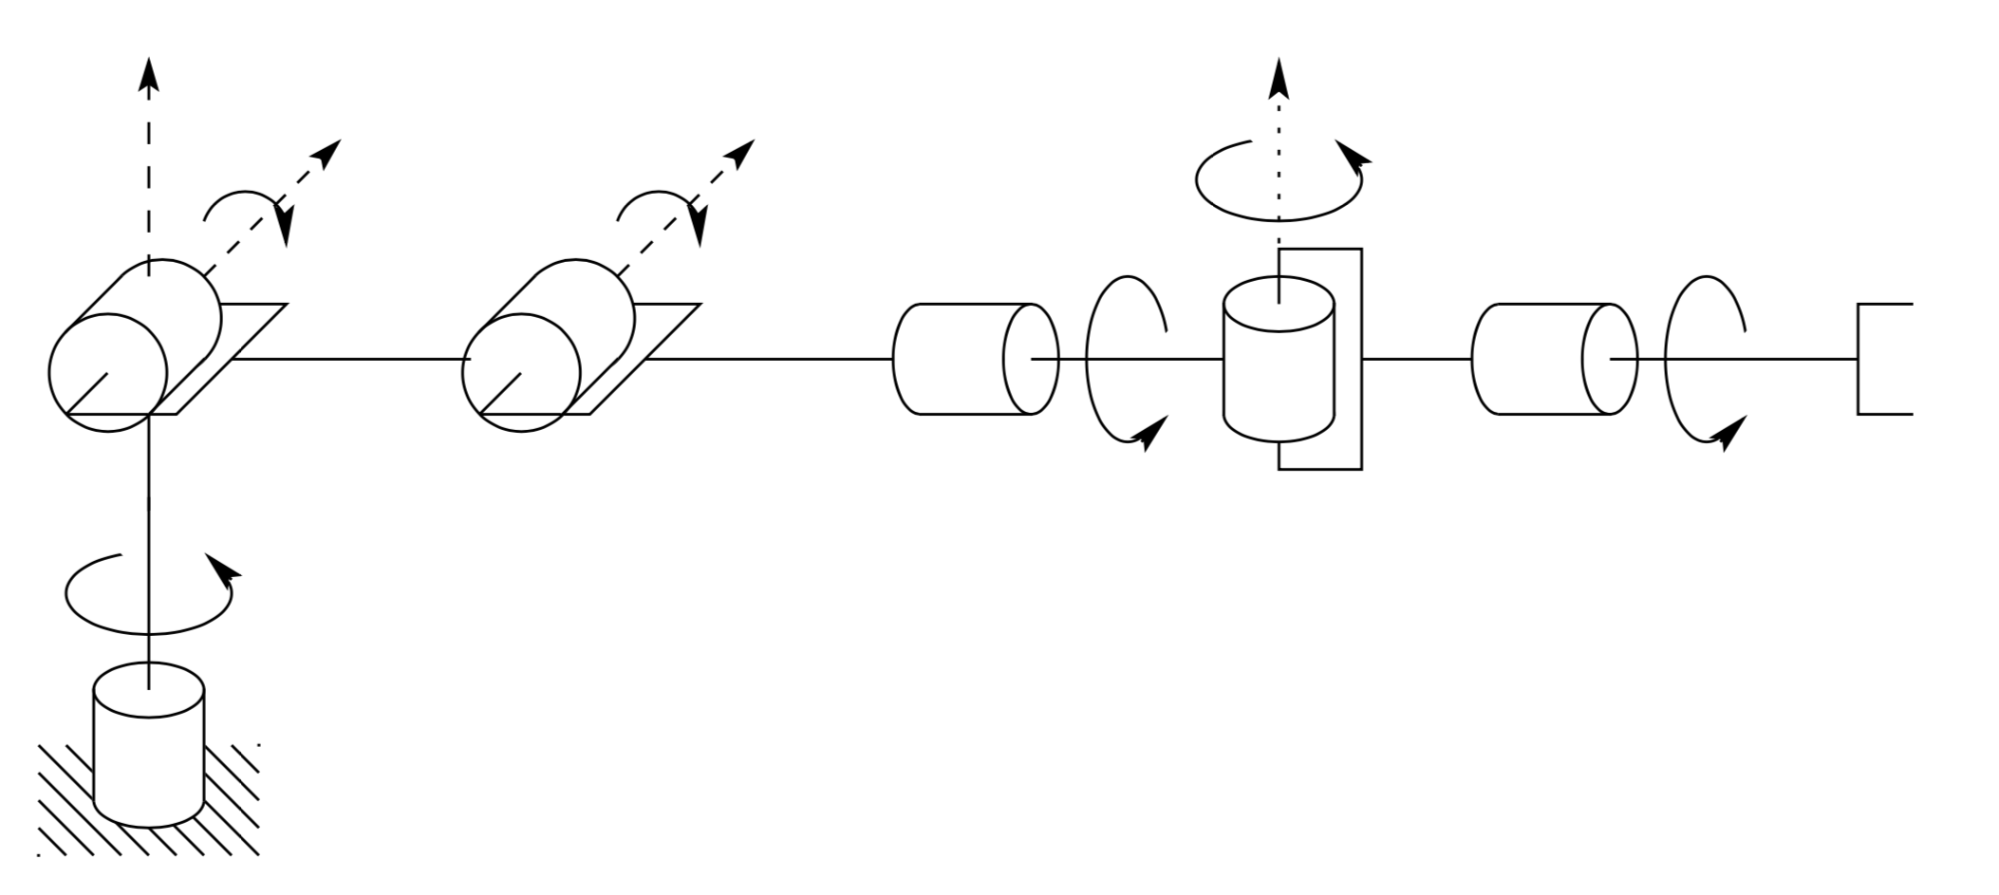
\includegraphics[width=.65\textwidth]{MEIOSISKinematicModel}
  \caption{MEIOSIS Kinematic Model \cite{robo}}
  \label{fig:MEIOSISKinematicModel}
\end{figure}

The model given in Figure \ref{fig:MEIOSISKinematicModel} represents the kinematics of a six degree of freedom manipulator. The body-attached frames affixed to each link were not configured using the Denavit-Hartenberg convention; rather they were aligned to allow for convenient and simple kinematic equations. The configuration of the last three links represent a spherical wrist, meaning that the inverse kinematics can be decoupled into position and orientation inverse kinematics problems. Including a spherical wrist in this configuration also allows the manipulator to be dexterous, meeting requirement 1.2.
